\chapter{实验结果与分析}\label{chap:experiment}

\section{实验设置}

所有 LeNet5 垃圾分类实验均采用官方 train/test 划分，训练集 2593 张，验证集 260 张。输入图片统一转灰度并 resize 到 $32\times32$。优化器使用 Adam，垃圾分类实验统一训练 24 个 epoch，batch size 为 32，学习率为 $1\times10^{-3}$，权重衰减为 $1\times10^{-4}$。LoRA 实验设置 rank 为 4，alpha 为 8。

\section{MNIST 预训练结果}

LeNet5 在 MNIST 上训练 5 个 epoch，结果如\cref{tab:mnist_result} 所示。测试准确率达到 98.60\%，说明模型实现和训练流程正确，生成的 \texttt{checkpoints/lenet\_mnist.ckpt} 可作为后续垃圾分类微调的初始化。

\begin{table}[!htb]
  \centering
  \caption{LeNet5 在 MNIST 上的预训练结果}
  \label{tab:mnist_result}
  \begin{tabular}{@{}lrrrrr@{}}
    \toprule
    \textbf{实验} & \textbf{训练样本} & \textbf{测试样本} & \textbf{可训练参数} & \textbf{时间} & \textbf{准确率} \\
    \midrule
    LeNet5 + MNIST 从零训练 & 60000 & 10000 & 61684 & 266.77 s & 98.60\% \\
    \bottomrule
  \end{tabular}
\end{table}

\begin{figure}[!htb]
  \centering
  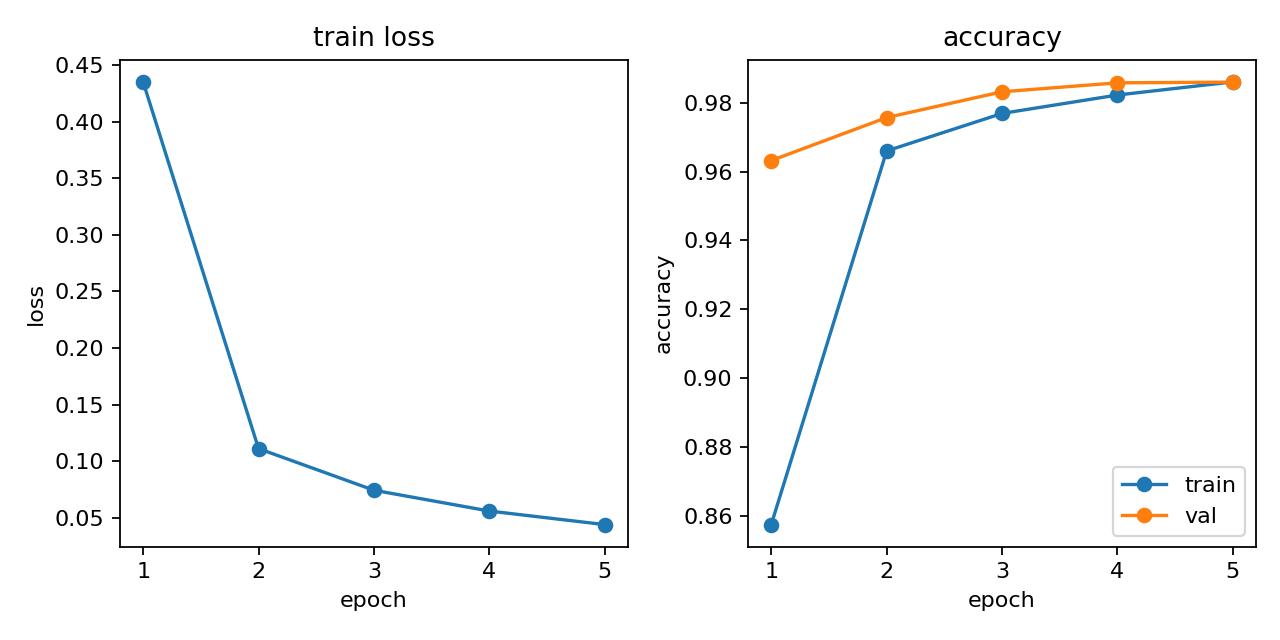
\includegraphics[width=0.86\linewidth]{figures/curve_lenet_mnist.png}
  \caption{LeNet5 在 MNIST 上的训练曲线}
  \label{fig:curve_mnist}
\end{figure}

\section{LeNet5 垃圾分类实验}

垃圾分类四组对比实验结果如\cref{tab:garbage_compare} 所示。

\begin{table}[!htb]
  \centering
  \caption{LeNet5 垃圾分类训练与微调结果}
  \label{tab:garbage_compare}
  \small
  \begin{tabular}{@{}lrrrrr@{}}
    \toprule
    \textbf{实验} & \textbf{可训练参数} & \textbf{总参数} & \textbf{时间} & \textbf{峰值显存} & \textbf{准确率} \\
    \midrule
    从零训练 & 63044 & 63044 & 362.80 s & 3698 MB & 3.85\% \\
    冻结微调 & 2210 & 63044 & 376.04 s & 3610 MB & 15.38\% \\
    全量微调 & 63044 & 63044 & 362.99 s & 3698 MB & 64.23\% \\
    LoRA 微调 & 5106 & 65940 & 379.66 s & 3610 MB & 25.38\% \\
    \bottomrule
  \end{tabular}
\end{table}

从零训练准确率仅为 3.85\%，接近 26 类随机猜测水平，说明小规模垃圾分类数据不足以让 LeNet5 从随机初始化中快速学到稳定特征。冻结微调将准确率提升到 15.38\%，说明 MNIST 预训练权重有一定帮助，但仅训练最后分类层的适应能力仍有限。

全量微调达到 64.23\%，是四组对比实验中最佳结果。原因在于所有卷积层和全连接层都可以根据垃圾分类图片重新调整，能够弥补 MNIST 与垃圾分类之间的分布差异。LoRA 微调的可训练参数为 5106，显存为 3610 MB，准确率为 25.38\%，高于冻结微调但低于全量微调。

需要务实指出的是，LeNet5 总参数量很小，全量微调与 LoRA 微调的峰值显存只相差 88 MB，训练时间也没有减少，LoRA 反而略慢。因此在 LeNet5 这种轻量网络上，LoRA 的实际工程收益很有限。本实验中 LoRA 的意义主要在于验证低秩分支插入、主干冻结和增量参数训练的实现流程，而不是证明 LoRA 在小模型上具有实用性能优势。

\section{训练曲线}

\begin{figure}[!htb]
  \centering
  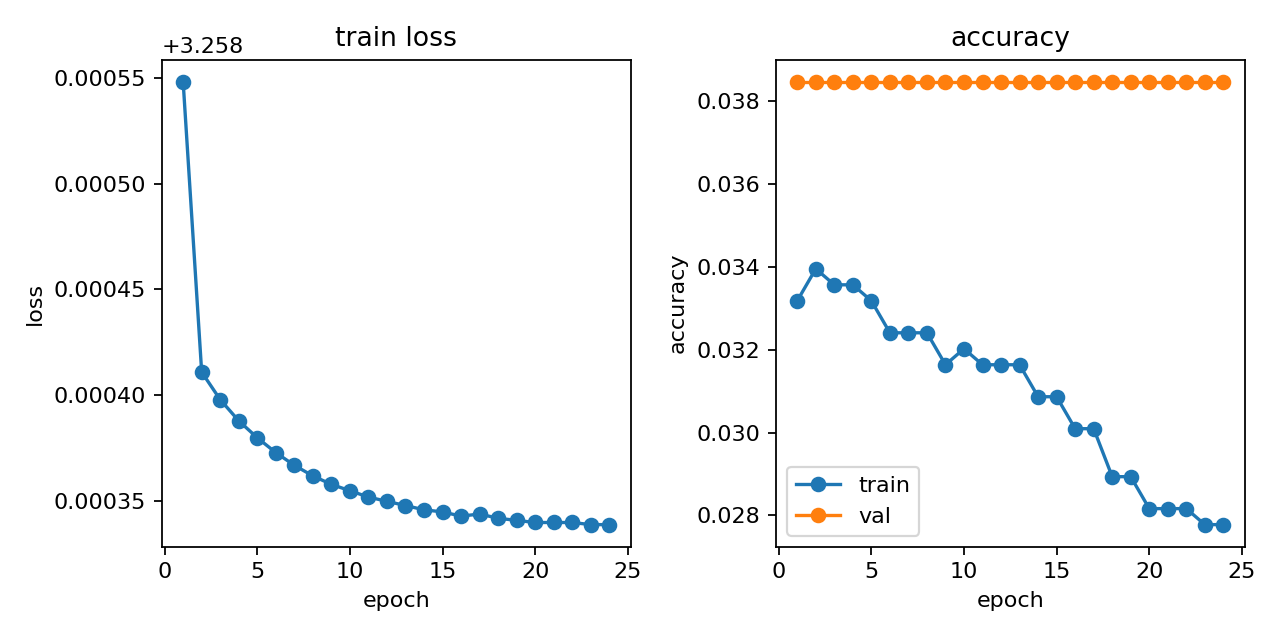
\includegraphics[width=0.82\linewidth]{figures/curve_lenet_garbage_scratch.png}
  \caption{LeNet5 垃圾分类从零训练曲线}
  \label{fig:curve_scratch}
\end{figure}

\begin{figure}[!htb]
  \centering
  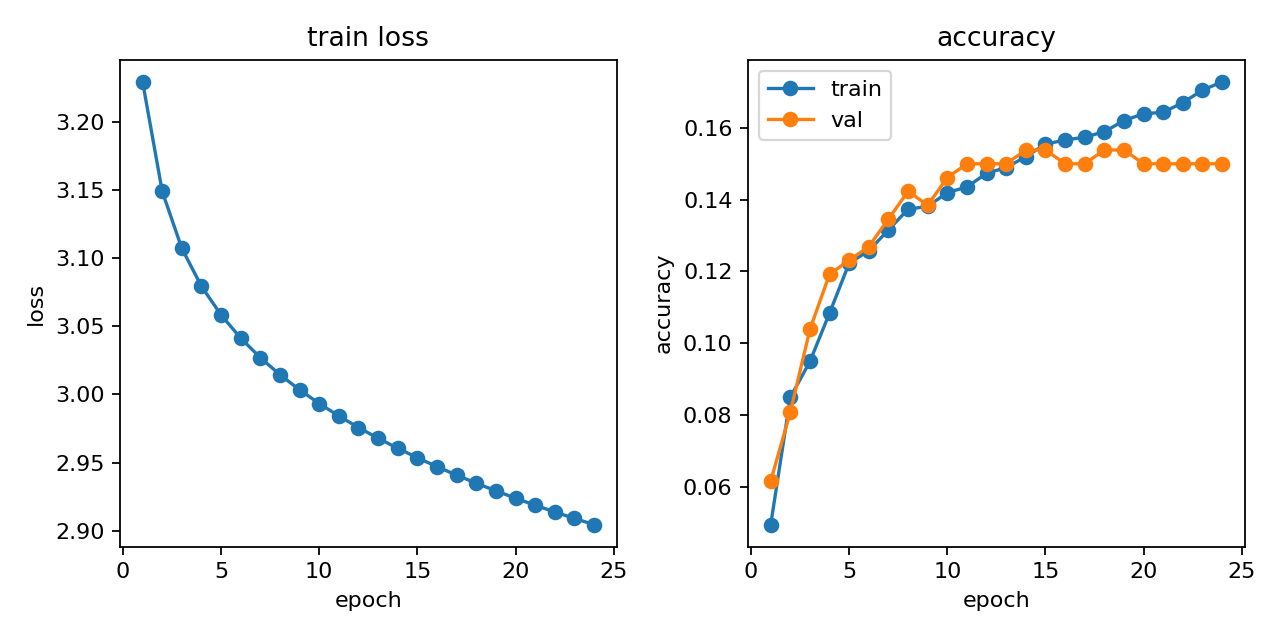
\includegraphics[width=0.82\linewidth]{figures/curve_lenet_garbage_freeze.png}
  \caption{LeNet5 垃圾分类冻结微调曲线}
  \label{fig:curve_freeze}
\end{figure}

\begin{figure}[!htb]
  \centering
  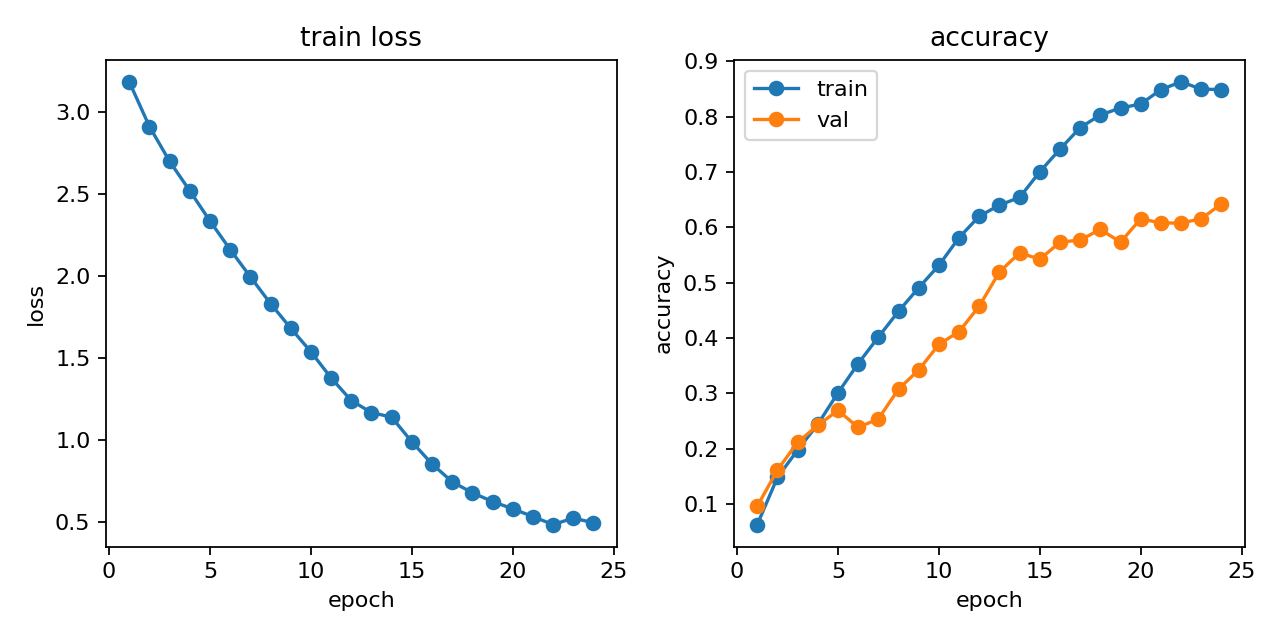
\includegraphics[width=0.82\linewidth]{figures/curve_lenet_garbage_full.png}
  \caption{LeNet5 垃圾分类全量微调曲线}
  \label{fig:curve_full}
\end{figure}

\begin{figure}[!htb]
  \centering
  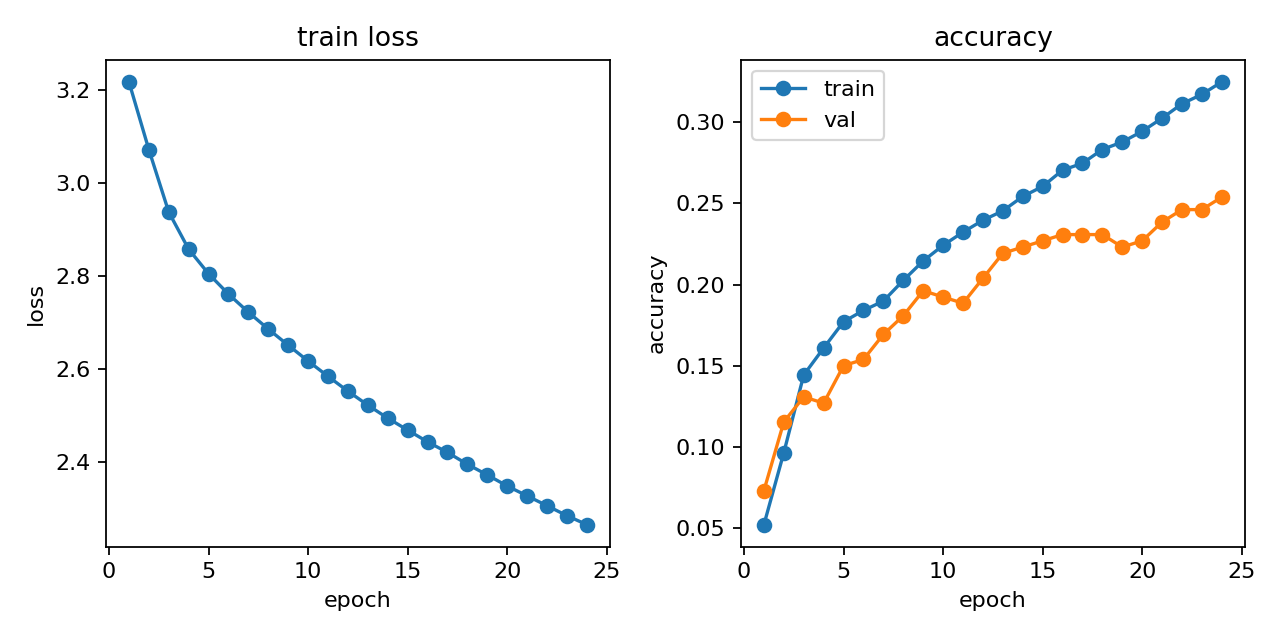
\includegraphics[width=0.82\linewidth]{figures/curve_lenet_garbage_lora.png}
  \caption{LeNet5 垃圾分类 LoRA 微调曲线}
  \label{fig:curve_lora}
\end{figure}

\section{模型改进实验}

模型改进实验在全量微调基础上启用 \texttt{--strong\_aug}，即增加随机旋转和随机水平翻转。除增强项外，epoch、batch size、学习率、权重衰减、输入尺寸和随机种子均保持一致。结果如\cref{tab:aug_compare} 所示。

\begin{table}[!htb]
  \centering
  \caption{强数据增强改进实验}
  \label{tab:aug_compare}
  \begin{tabular}{@{}lrrrr@{}}
    \toprule
    \textbf{实验} & \textbf{改动} & \textbf{可训练参数} & \textbf{时间} & \textbf{准确率} \\
    \midrule
    全量微调基线 & 默认预处理 & 63044 & 362.99 s & 64.23\% \\
    强数据增强 & 随机旋转 + 水平翻转 & 63044 & 364.80 s & 38.85\% \\
    \bottomrule
  \end{tabular}
\end{table}

\begin{figure}[!htb]
  \centering
  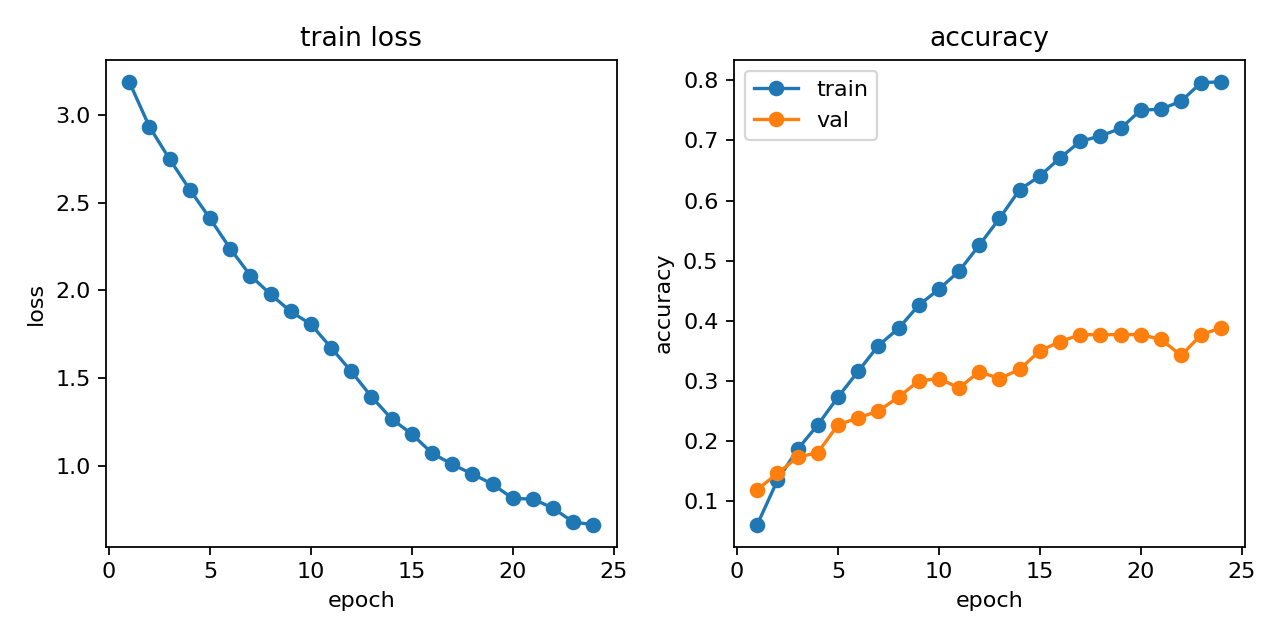
\includegraphics[width=0.82\linewidth]{figures/curve_lenet_garbage_full_aug.png}
  \caption{LeNet5 强数据增强改进实验曲线}
  \label{fig:curve_aug}
\end{figure}

强数据增强没有带来提升，准确率从 64.23\% 降至 38.85\%。这不是一个可以简单解释为“增强不适合垃圾分类”的结果，因为水平翻转和适度旋转通常属于保持标签不变的数据增强。为排查原因，本文额外保存了增强前后的输入可视化，如\cref{fig:preprocess_preview} 所示。

\begin{figure}[!htb]
  \centering
  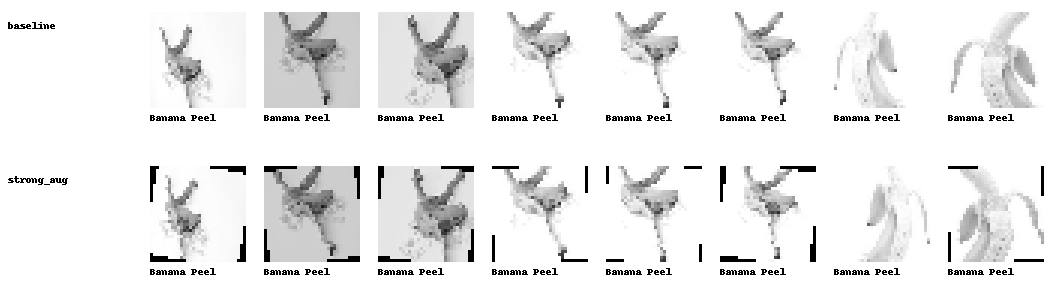
\includegraphics[width=0.92\linewidth]{figures/preprocess_lenet_preview.png}
  \caption{LeNet5 输入预处理可视化：baseline 与 strong\_aug 对比}
  \label{fig:preprocess_preview}
\end{figure}

可视化结果显示，随机旋转后的 $32\times32$ 灰度图出现了明显黑色边框。由于 LeNet5 输入尺寸很小，这些边框在图像中占比较高，可能成为与类别无关的强伪特征，干扰模型学习。更合理的做法是调整旋转填充值、使用中心裁剪/反射填充，或先在更高分辨率下增强再缩放。因此本文将该实验视为一次负向消融：它暴露了增强算子配置与低分辨率输入之间的冲突，而不是说明数据增强思想本身无效。

\section{综合分析}

从准确率看，全量微调明显优于冻结微调和 LoRA 微调，说明当前任务需要更新全部 LeNet5 参数以适配真实垃圾图片。从可训练参数看，冻结微调最省参数，仅 2210 个；LoRA 微调为 5106 个，在显存占用与冻结微调相近的情况下取得更高准确率；全量微调参数最多，但由于 LeNet5 规模较小，训练成本仍可接受。

从显存看，冻结微调和 LoRA 微调峰值显存为 3610 MB，低于全量微调和从零训练的 3698 MB，但差距只有 88 MB。训练时间差异也不大，主要受数据加载和容器开销影响。综合而言，在 LeNet5 这种小模型上，全量微调是准确率最优策略；LoRA 的工程节省并不明显，更适合作为参数高效微调机制的实现验证；冻结微调适合作为低成本基线。

\section{进阶对照实验：MobileNetV2}

LeNet5 实验完成了从 MNIST 预训练到垃圾分类微调的完整链路，适合观察卷积层、全连接层、冻结策略和 LoRA 分支的具体作用。但从真实垃圾分类任务本身看，LeNet5 的输入被压缩为 $32\times32$ 灰度图，模型容量也较小，容易形成性能上限。为进一步回答“如果使用课程资料中更接近实际应用的轻量级网络，垃圾分类可以达到什么水平”，本文加入 MobileNetV2 进阶对照实验。

MobileNetV2 对照实验和 LeNet5 的关键差异有三点。第一，输入保持 RGB 三通道并 resize 到 $224\times224$，能够保留颜色和更丰富的局部纹理；第二，网络由倒残差模块和 depthwise separable convolution 组成，参数量明显高于 LeNet5，但仍属于轻量级 CNN；第三，官方 ImageNet 预训练权重提供了大规模自然图像上的通用视觉特征。通过这组实验，可以判断 LeNet5 结果到底受限于训练流程，还是受限于输入适配和模型表达能力。

MobileNetV2 对照实验分为两条线。第一条线是自实现 MobileNetV2，用于观察在没有完整匹配官方预训练权重时，大模型是否自然优于小模型。第二条线是 MindCV 官方 MobileNetV2，用于观察结构、参数名和预训练 checkpoint 完整匹配时，迁移学习在垃圾分类上的实际表现。

\subsection{自实现 MobileNetV2 基线}

自实现 MobileNetV2 使用 RGB 输入和 $224\times224$ 分辨率，参数量约 229 万。该模型主要由 ConvBNReLU、InvertedResidual 和全局平均池化分类头组成。与 LeNet5 不同，它保留了 RGB 颜色信息，并使用 ImageNet 常用均值和标准差归一化。

未加载完整匹配的官方预训练权重时，三种策略结果如\cref{tab:mobile_self} 所示。

\begin{table}[!htb]
  \centering
  \caption{自实现 MobileNetV2 基线结果}
  \label{tab:mobile_self}
  \small
  \begin{tabular}{@{}lrrrr@{}}
    \toprule
    \textbf{策略} & \textbf{可训练参数} & \textbf{总参数} & \textbf{时间} & \textbf{准确率} \\
    \midrule
    freeze & 33306 & 2291290 & 328.15 s & 17.31\% \\
    full & 2291290 & 2291290 & 544.21 s & 51.92\% \\
    LoRA & 107418 & 2365402 & 550.82 s & 40.38\% \\
    \bottomrule
  \end{tabular}
\end{table}

这组结果说明，更大的网络如果缺少高质量初始化，并不必然优于 LeNet5。自实现 MobileNetV2 全量微调为 51.92\%，低于 LeNet5 全量微调的 64.23\%。其原因主要有两点：一是垃圾分类训练集只有 2593 张，较大模型从随机或不充分预训练状态开始训练时更容易受数据规模限制；二是 MobileNetV2 依赖 BatchNorm、倒残差堆叠和更深层特征传递，如果预训练权重未完整匹配，早期训练阶段的特征分布不稳定。

冻结微调只有 17.31\%，说明未充分预训练的 backbone 不能直接作为特征提取器。此时只训练最后分类头，相当于用一组质量不高且不可更新的特征做线性分类，上限自然很低。LoRA 达到 40.38\%，高于冻结但低于全量，说明在较大网络中低秩分支比只训练分类头更灵活，可以对中后层特征进行一定修正；但在缺少高质量预训练表示时，LoRA 仍然无法完全替代全量参数更新。

因此，自实现 MobileNetV2 的价值不在于取得最高准确率，而在于说明迁移学习不是“模型越大越好”的简单问题。模型结构、预训练权重、参数加载匹配程度和学习率策略必须同时成立，才能发挥现代 CNN 的优势。

\subsection{MindCV 官方预训练 MobileNetV2}

进一步使用 MindCV 官方 MobileNetV2-1.0，并加载匹配的 ImageNet 预训练 checkpoint。与自实现模型相比，官方模型的结构定义、参数命名和 checkpoint 对齐程度更高，能够加载 260 个匹配参数。实验同样比较冻结微调、全量微调和 LoRA 微调，并额外测试了常量学习率与 warmup + cosine 学习率调度的差异。结果如\cref{tab:mobile_mindcv} 所示。

\begin{table}[!htb]
  \centering
  \caption{MindCV 官方预训练 MobileNetV2-1.0 结果}
  \label{tab:mobile_mindcv}
  \small
  \begin{tabular}{@{}lrrrr@{}}
    \toprule
    \textbf{策略} & \textbf{LR 策略} & \textbf{可训练参数} & \textbf{时间} & \textbf{准确率} \\
    \midrule
    freeze & constant & 33306 & 378.99 s & 87.31\% \\
    full & constant & 2291290 & 627.08 s & 8.08\% \\
    full & cosine + warmup & 2291290 & 622.66 s & 91.15\% \\
    LoRA & constant & 80922 & 459.41 s & 89.62\% \\
    \bottomrule
  \end{tabular}
\end{table}

官方预训练 MobileNetV2 的结果显著高于 LeNet5。冻结微调已达到 87.31\%，说明 ImageNet 预训练 backbone 已经具备较强的通用特征提取能力，即使只替换并训练最后分类头，也能较好地区分 26 类垃圾图像。LoRA 微调达到 89.62\%，在只训练约 8.1 万参数的情况下进一步超过冻结微调，说明低秩分支能够在保留主干预训练特征的同时，对垃圾分类的高层语义表示进行轻量修正。全量微调配合 warmup + cosine 学习率衰减达到 91.15\%，是所有实验中最高的结果，说明当优化策略合适时，开放全部参数可以进一步提高模型对目标数据分布的适配能力。

值得注意的是，full constant 只有 8.08\%，远低于 freeze 和 LoRA。这个结果说明预训练模型全量微调不能简单使用固定学习率直接训练。全量开放参数后，反向传播会同时改变低层边缘纹理特征和高层语义特征；如果学习率调度不稳，模型可能在前几个 epoch 快速破坏原有预训练表示，导致验证准确率崩溃。相比之下，warmup + cosine 先用较小步长平稳适配新分类头和中高层特征，再逐步衰减学习率，有利于在“保留通用特征”和“适配新任务”之间取得平衡。

从任务角度看，这组结果还说明垃圾分类图片中颜色和分辨率非常重要。例如塑料、金属、纸张、果皮等类别不仅依赖形状轮廓，也依赖颜色、反光、纹理和局部细节。LeNet5 为了适配 MNIST 预训练链路将图片灰度化并压缩到 $32\times32$，便于完成可解释的迁移学习实验；MobileNetV2 则保留更接近真实视觉任务的输入形态，因此能显著提高准确率。

\begin{figure}[!htb]
  \centering
  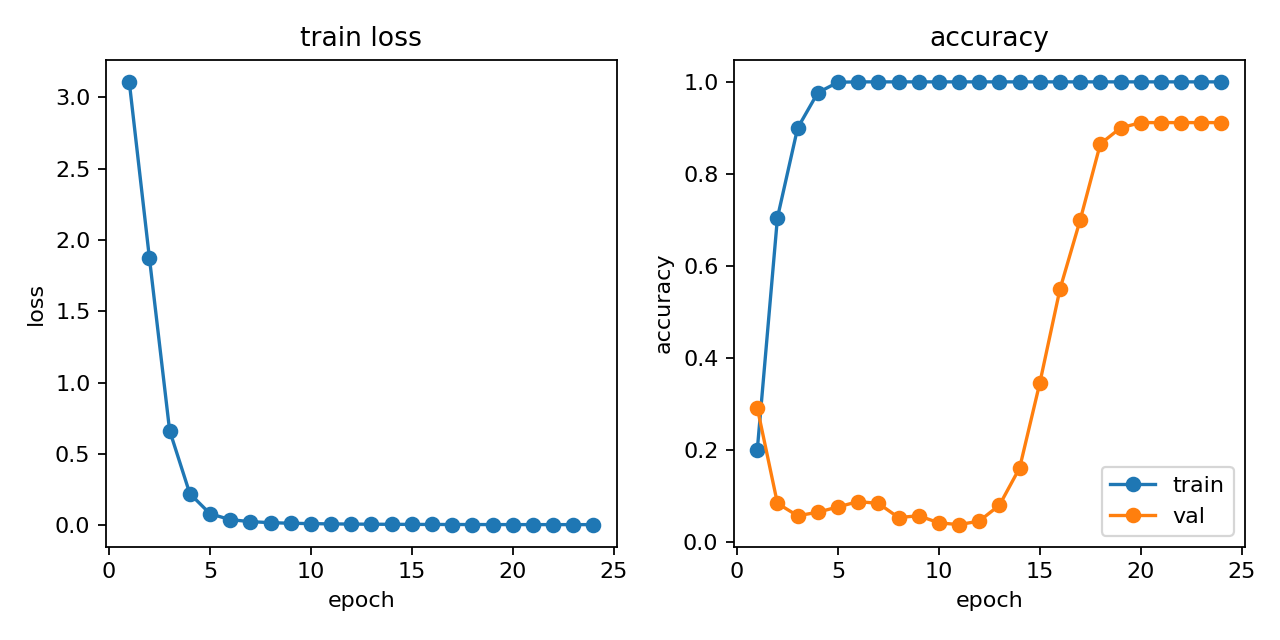
\includegraphics[width=0.82\linewidth]{figures/curve_mindcv_mobilenet_v2_100_full_cosine.png}
  \caption{MindCV MobileNetV2-1.0 full + cosine 训练曲线}
  \label{fig:mobile_full_cosine}
\end{figure}

\begin{figure}[!htb]
  \centering
  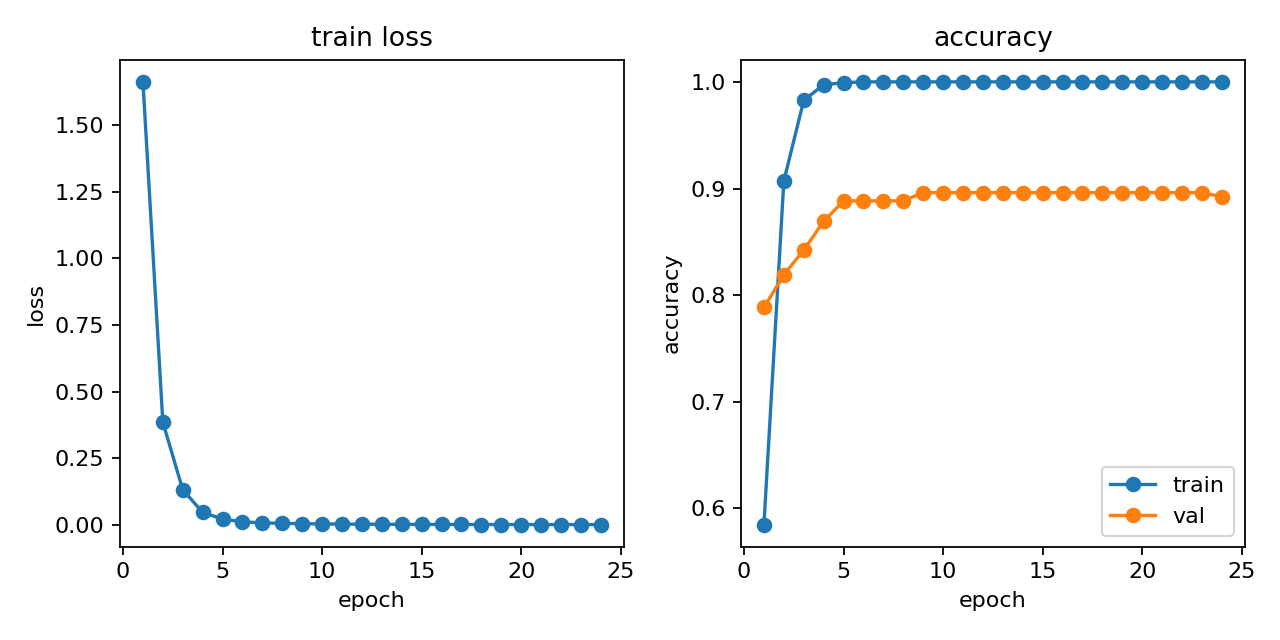
\includegraphics[width=0.82\linewidth]{figures/curve_mindcv_mobilenet_v2_100_lora_real.png}
  \caption{MindCV MobileNetV2-1.0 LoRA 微调曲线}
  \label{fig:mobile_lora}
\end{figure}

\subsection{MobileNetV2 中 LoRA 的意义}

LeNet5 上的 LoRA 边际收益有限，因为模型本身只有约 6.3 万参数。MobileNetV2 上的 LoRA 更能体现参数高效微调的意义：MindCV MobileNetV2-1.0 LoRA 只训练约 8.1 万参数，准确率达到 89.62\%，接近全量 cosine 微调的 91.15\%，同时训练时间为 459.41 s，低于全量 cosine 的 622.66 s。

在该实验中，LoRA 主要插入到 MobileNetV2 后部的 $1\times1$ pointwise convolution 层。这些层负责通道混合和高层语义特征调整，适合用低秩分支进行轻量适配。设原卷积或线性映射的权重更新为 $\Delta W$，LoRA 用两个低秩矩阵近似该更新，即 $\Delta W=BA\cdot\alpha/r$，从而避免直接训练完整权重矩阵。对于 MobileNetV2 这类参数量百万级的网络，LoRA 可以明显减少可训练参数量，并降低优化时需要保存的梯度和优化器状态。

这也解释了 LeNet5 与 MobileNetV2 中 LoRA 表现的差异。LeNet5 参数太少，全量微调本身成本已经很低，LoRA 的节省空间有限；而 MobileNetV2 参数规模更大，且预训练特征更强，冻结主干后只给中后层增加低秩可训练分支，就能在较低训练成本下接近全量微调精度。因此，LeNet5 中的 LoRA 更偏向方法实现验证，MobileNetV2 中的 LoRA 更能体现参数高效微调的实际价值。

\subsection{MobileNetV2-0.75 宽度版本实验}

为了进一步观察模型宽度对迁移学习效果的影响，本文还测试了 MindCV MobileNetV2-0.75。该模型将通道宽度缩小，总参数约 141 万，低于 MobileNetV2-1.0 的约 229 万。结果如\cref{tab:mobile_075} 所示。

\begin{table}[!htb]
  \centering
  \caption{MindCV MobileNetV2-0.75 补充实验结果}
  \label{tab:mobile_075}
  \small
  \begin{tabular}{@{}lrrrr@{}}
    \toprule
    \textbf{策略} & \textbf{可训练参数} & \textbf{时间} & \textbf{峰值显存} & \textbf{准确率} \\
    \midrule
    freeze & 33306 & 378.74 s & 3367 MB & 83.85\% \\
    full constant & 1415370 & 553.01 s & 4453 MB & 17.31\% \\
    full cosine & 1415370 & 576.85 s & 4453 MB & 90.77\% \\
    LoRA & 70298 & 395.93 s & 3429 MB & 87.69\% \\
    \bottomrule
  \end{tabular}
\end{table}

0.75 版本的结果与 1.0 版本总体一致：冻结和 LoRA 在完整预训练权重下表现稳定，全量微调必须配合学习率衰减；常量学习率全量微调明显不可靠。full cosine 达到 90.77\%，略低于 1.0 版本的 91.15\%，说明在该数据集规模下，缩小网络宽度只带来有限准确率损失。LoRA 达到 87.69\%，低于 1.0 版本 LoRA 的 89.62\%，但仍明显高于 LeNet5 和自实现 MobileNetV2，说明高质量预训练权重比单纯增加或减少网络宽度更关键。

从资源消耗看，0.75 版本 full cosine 的峰值显存为 4453 MB，高于 freeze 和 LoRA 的 3367 MB、3429 MB。LoRA 在保持较高准确率的同时，显存更接近冻结微调，这与参数高效微调的设计目标一致。该结果也补充说明：当模型规模增大后，冻结、LoRA、全量微调在资源占用上的差异会比 LeNet5 更明显。

\subsection{与 LeNet5 实验的互补关系}

MobileNetV2 进阶对照实验使本文结论更完整。LeNet5 适合完成课程设计中的基础迁移学习链路：先在 MNIST 上训练，再迁移到垃圾分类，并分别比较从零训练、冻结微调、全量微调和 LoRA 微调。由于 LeNet5 结构简单、层次清晰，冻结哪些层、训练哪些层、LoRA 加在哪些层都容易解释。

MobileNetV2 则从真实应用角度补充说明：如果目标是提高垃圾分类准确率，应尽量保留颜色信息、使用更高输入分辨率，并加载与模型结构匹配的高质量预训练权重。从结果看，LeNet5 全量微调 64.23\% 已经说明 MNIST 初始化具有一定价值，但模型受限明显；MindCV MobileNetV2-1.0 full + cosine 达到 91.15\%，说明垃圾分类任务本身并非不可学，而是 LeNet5 的输入适配和模型容量限制了上限。

因此，两组实验并不是互相替代的关系。LeNet5 回答“迁移学习、冻结微调和 LoRA 如何在一个可控的小型 CNN 中实现”，MobileNetV2 回答“在更接近实际视觉任务的输入和预训练条件下，垃圾分类性能可以提升到什么程度”。前者保证实验机制清楚，后者使结果分析更贴近真实应用。
